\begin{figure}[htbp]
\centering
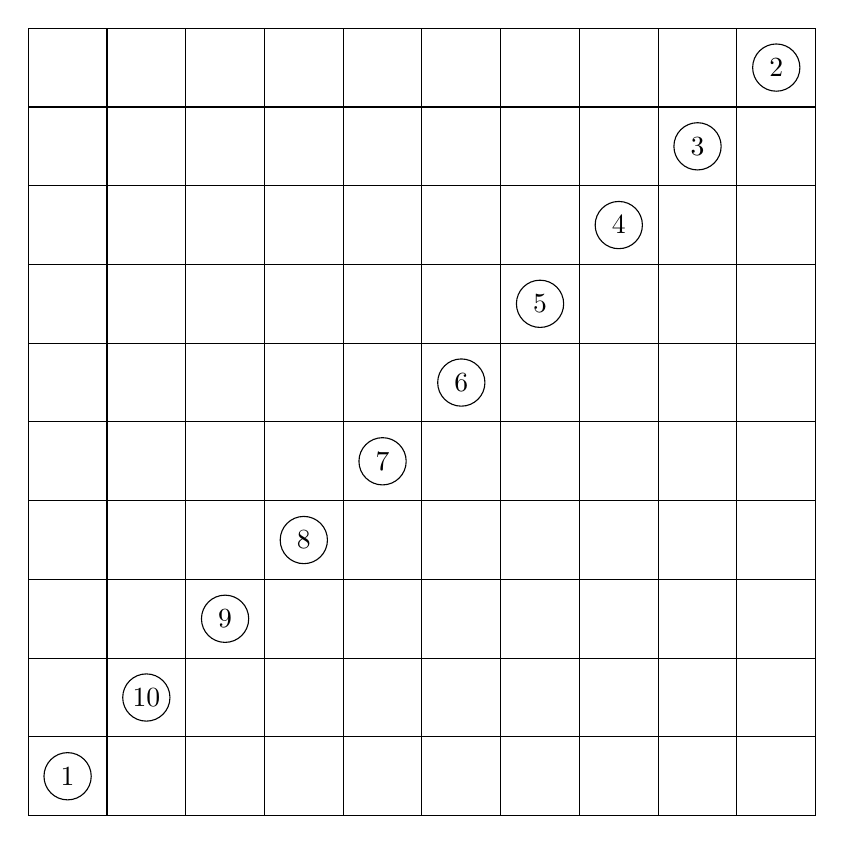
\begin{tikzpicture}

	\draw[xshift=0.5cm, yshift=0.5cm] (0,0) grid (10,10);
	\draw (1, 1) circle [radius=0.3];
	\draw (2, 2) circle [radius=0.3];
	\draw (3, 3) circle [radius=0.3];
	\draw (4, 4)  circle [radius=0.3];
	\draw (5, 5)  circle [radius=0.3];
	\draw (6, 6) circle [radius=0.3];
	\draw (7, 7)  circle [radius=0.3];
	\draw (8, 8)  circle [radius=0.3];
	\draw (9, 9)  circle [radius=0.3];
	\draw (10, 10)  circle [radius=0.3];

	\draw (1, 1) node {1};
	\draw (2, 2) node {10};
	\draw (3, 3) node{9};
	\draw (4, 4) node{8};
	\draw (5, 5) node{7};
	\draw (6, 6) node{6};
	\draw (7, 7) node{5};
	\draw (8, 8) node{4};
	\draw (9, 9) node{3};
	\draw (10, 10) node{2};
	
\end{tikzpicture}

\emph{Se tiene 1 central disponible}

\caption{Caso de peor entrada con las 10 ciudades y 1 central}
\label{ej_2:peor}
\end{figure}
